\begin{figure}[htbp]
  \centering
  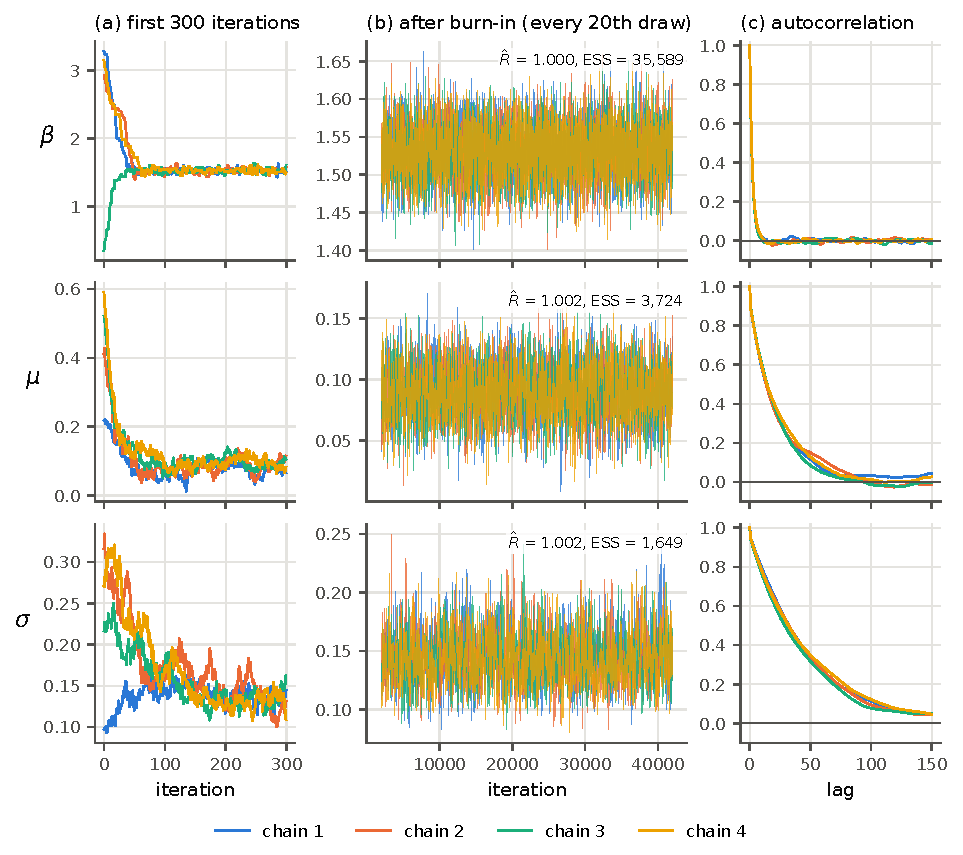
\includegraphics[width=\linewidth]{trace.pdf}
  \caption{Convergence of the sampler on the real data: 4 chains started from points drawn from the prior. (a): the first 300 iterations, where the chains leave their dispersed starting points and meet long before the end of the burn-in of 2,000 iterations. (b): the 40,000 iterations kept per chain after burn-in, which overlap, with the split-$\hat R$ and the effective sample size (ESS) of the four chains together. (c): autocorrelation of each chain after burn-in. $\beta$ mixes fast; $\mu$ and especially $\sigma$ are more autocorrelated, because they move only through the 359 opening effects, but their ESS of 3,724 and 1,649 still make the Monte Carlo errors small compared with the posterior standard deviations.}
  \label{fig:trace}
\end{figure}
